\chapter{Data analysis and results}
\label{chapter:data_analysis_results}

\section{Data source}

Given all threads from Hack Forums Market section, each document is a mix of data: Thread heading and First post content and timestamp.\\
All threads from sub-forums in Market section have been pre-processed. Two datasets have been built by filtering all DDoS related threads:
\begin{itemize}
    \item \textit{ddos\_full\_dataset.csv}: ($>$40K docs, full dataset with all market section documents related with IoT DDoS.
    \item \textit{ddos\_groundtruth\_dataset.csv}: (4K docs), data sample. Randomly extracted from full dataset. Every doc category has been annotated by differenciating beteen \textit{supply} and \textit{demand}. This dataset is intended for training and testing text classification models.
\end{itemize}

All contents have been cleaned when building the datasets. Cleaning operations have been:
\begin{itemize}
    \item Lower case all text.
    \item Removed: punctuation, accents, non-textual content like citing, images, urls, ...
\end{itemize}

Ground truth dataset preview can be shown in figure \ref{fig:ground_truth_preview}.

\begin{figure}[H]
	\centering
	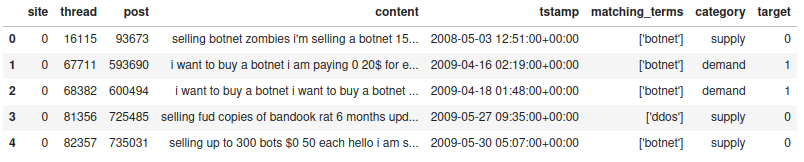
\includegraphics[width=1.0\textwidth]{figs/ground_truth_preview.png}
	\caption{Ground truth data preview}
	\label{fig:ground_truth_preview}
\end{figure}

Ground truth dataset has been split in two datasets for training and testing with 80/20 ratio. Resulting datasets have 3257 documents and 814 documents respectively.

\section{Data pre-process}

Since there are a lot of different words in corpus, result is a high dimensional dataset (too much different features). Building feature vectors with full word list is inefficient and can be unmanageable. This is why only non-zero parts of feature vectors are maintained in memory during analysis process. Main purpose of data pre-process phase is to reduce dataset dimensions. To do that, \textit{Tokenization} and \textit{Term Frequency calculations} techniques have been applied to dataset.

\subsection{Tokenization}

It consists in breaking down text in term vectors and filtering stop words. \textit{CountVectorizer} \cite{CountVectorizer} sklearn text feature extraction tool has been used for that purpose. It converts a collection of text documents (ground truth dataset \textit{content} column) to a matrix of token counts. This implementation produces a sparse representation of the counts.

\subsection{Term Frequency}

Some thread contents are longer than others, it can result in a higher average count values than shorter ones, but they really talk about same topic (category). Among that, some words appears in many documents in the corpus. These common words are less informative, so downscaling weights for these words is needed. In order to avoid this problem, a calculation tf and tf-idf (\textit{Term Frequency times Inverse Document Frequency}) has been done. Both (tf and tf-idf) are computed by TfidfTransformer \cite{TfidfTransformer}, a tool from sklearn text feature extraction.

\section{Model training}
\label{sec:training}

Accuracy has been tested for four well-known classification models. These models are widely used in classification tasks:
\begin{itemize}
    \item LinearSVC: Linear Support Vector Classification \cite{hsu2003practical}.
    \item SGD: Stochastic Gradient Descent \cite{ketkar2017stochastic}.
    \item K nearest Neighbors \cite{kozma2008k}.
    \item Multinomial Naïve Bayes \cite{kibriya2004multinomial}.
\end{itemize}

Performance metrics to be analysed are: precision, recall, F1-score and occurrences of each class (support). Confusion matrix will show, for each model, ratio of correct and wrong classification between categories (only two categories in our case).

\subsection{LinearSVC}
\label{sec:LinearSVC}

LinearSVC classification model accuracy has been 0.96. Figure \ref{fig:LinearSVC_cfm} shows its confusion matrix.
\begin{figure}[H]
	\centering
	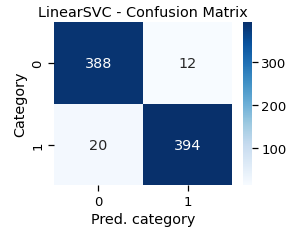
\includegraphics[width=0.3\textwidth]{figs/LinearSVC_cfm.png}
	\caption{LinearSVC confusion matrix}
	\label{fig:LinearSVC_cfm}
\end{figure}

\subsection{Stochastic Gradient Descent (SGD)}

Stochastic Gradient Descent classification model accuracy has been 0.93. Figure \ref{fig:sgd_cfm} shows its confusion matrix.
\begin{figure}[H]
	\centering
	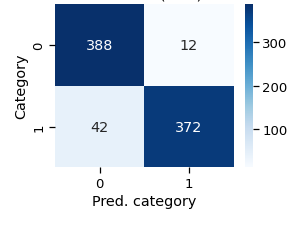
\includegraphics[width=0.3\textwidth]{figs/sgd_cfm.png}
	\caption{Stochastic Gradient Descent confusion matrix}
	\label{fig:sgd_cfm}
\end{figure}

\subsection{K-nearest neighbors}

K-nearest Neighbors classification model accuracy has been 0.79. Figure \ref{fig:knn_cfm} shows its confusion matrix.
\begin{figure}[H]
	\centering
	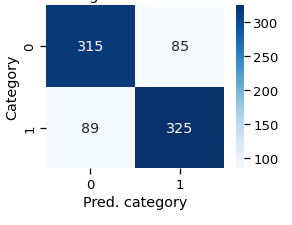
\includegraphics[width=0.3\textwidth]{figs/knn_cfm.png}
	\caption{K-nearest neighbors confusion matrix}
	\label{fig:knn_cfm}
\end{figure}

\subsection{Multinomial Naïve Bayes}

Multinomial Naïve Bayes classification model accuracy has been 0.89. Figure \ref{fig:mnb_cfm} shows its confusion matrix.
\begin{figure}[H]
	\centering
	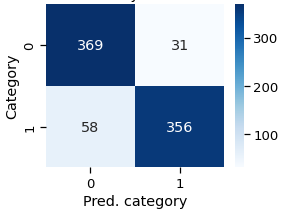
\includegraphics[width=0.3\textwidth]{figs/mnb_cfm.png}
	\caption{Multinomial Naïve Bayes confusion matrix}
	\label{fig:mnb_cfm}
\end{figure}

\section{Model evaluation}

\subsection{Metrics}

As stated in section \textit{Model training} \ref{sec:training}, performance metrics to be analysed are: precision, recall, F1-score and occurrences of each class (support). Results obtained in training stage are shown in figure \ref{fig:metrics}.

\begin{figure}[H]
	\centering
	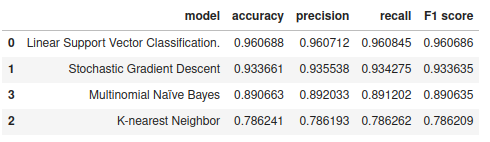
\includegraphics[width=0.7\textwidth]{figs/metrics.png}
	\caption{Training metrics report}
	\label{fig:metrics}
\end{figure}

\subsection{ROC curve}

The receiver operating characteristic (ROC) curve \cite{gonccalves2014roc} is frequently used for evaluating the performance of binary classification algorithms. It provides a graphical representation of a classifier’s performance, rather than a single value like most other metrics.

\begin{figure}[H]
	\centering
	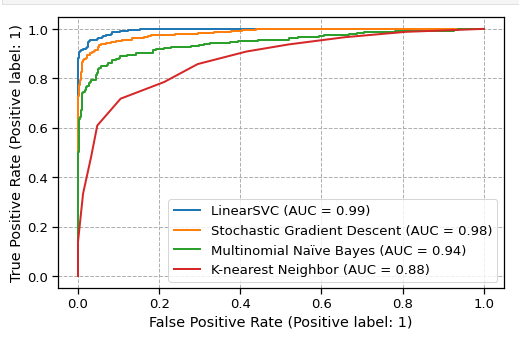
\includegraphics[width=0.7\textwidth]{figs/roc.png}
	\caption{ROC curve}
	\label{fig:roc}
\end{figure}

\subsection{Model selection}

According to evaluation results, best performing model is LinearSVC (Linear Support Vector Classifier) \ref{sec:LinearSVC}. Area under the curve in ROC curve figure \ref{fig:roc} and training metric values are close but better than Stochastic Gradient Descent model. The rest of the models clearly have worse results.

\section{Data Analysis}
\label{sec:analysis}

After selecting a prediction model, full dataset has been loaded and its documents have been labelled according to selected model prediciton results. An example on how documents have been labeled can is shown in figure \ref{fig:labels}

\begin{figure}[H]
	\centering
	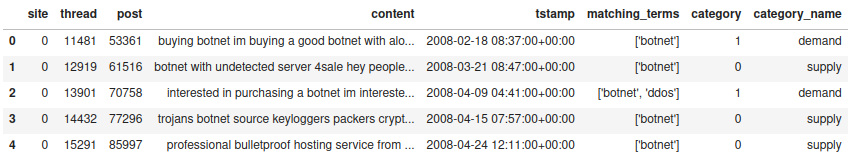
\includegraphics[width=1.0\textwidth]{figs/labels.png}
	\caption{Labeled documents example}
	\label{fig:labels}
\end{figure}

\subsection{Supply vs Demand}

Analysing evolution of supply and demand over time  allows to know how community members interest in that type of services have evolved of underground. It is the first step in analysing relevance of Sale of IoT devices for DDoS services in underground forums.

\begin{figure}[H]
	\centering
	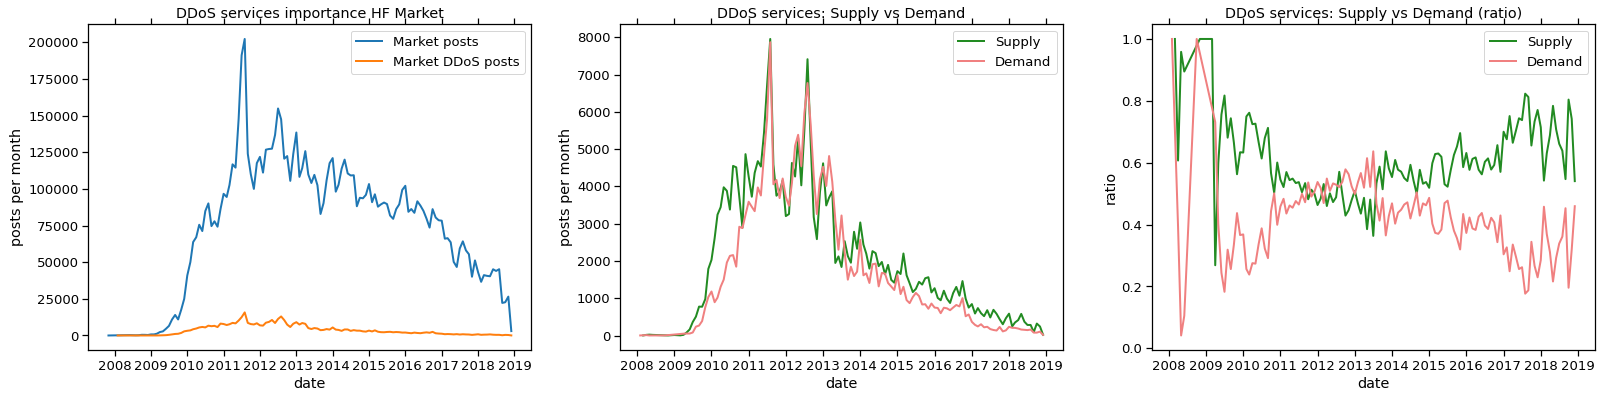
\includegraphics[width=1.0\textwidth]{figs/supply_vs_demand_full.png}
	\caption{Supply vs Demand posts volume in HF market}
	\label{fig:supply_vs_demand_full}
\end{figure}

As shown in fig. \ref{fig:supply_vs_demand_full}, supply did pass demand in 2012 and nowadays is clearly higher. However, according to results shown in fig. \ref{fig:terms} depending on the intention of the service, the demand may be higher than the supply. \\
This is happening today with \textit{stresser} related services. \textit{Stressers} are DDoS systems controlled by a professional operator. They are used to test the resistance of network systems against DDoS attacks.

\subsection{Relevant tech terms}

It is common to refer to \textit{Sale of access IoT devices services for DDoS} by using different tech terms like booter, stresser, ddoser, and so on. The use of some terms or others, when referring to these services, varies depending on the technology used to develop them, the intended use or simply the slang of the moment.

\begin{figure}[H]
	\centering
	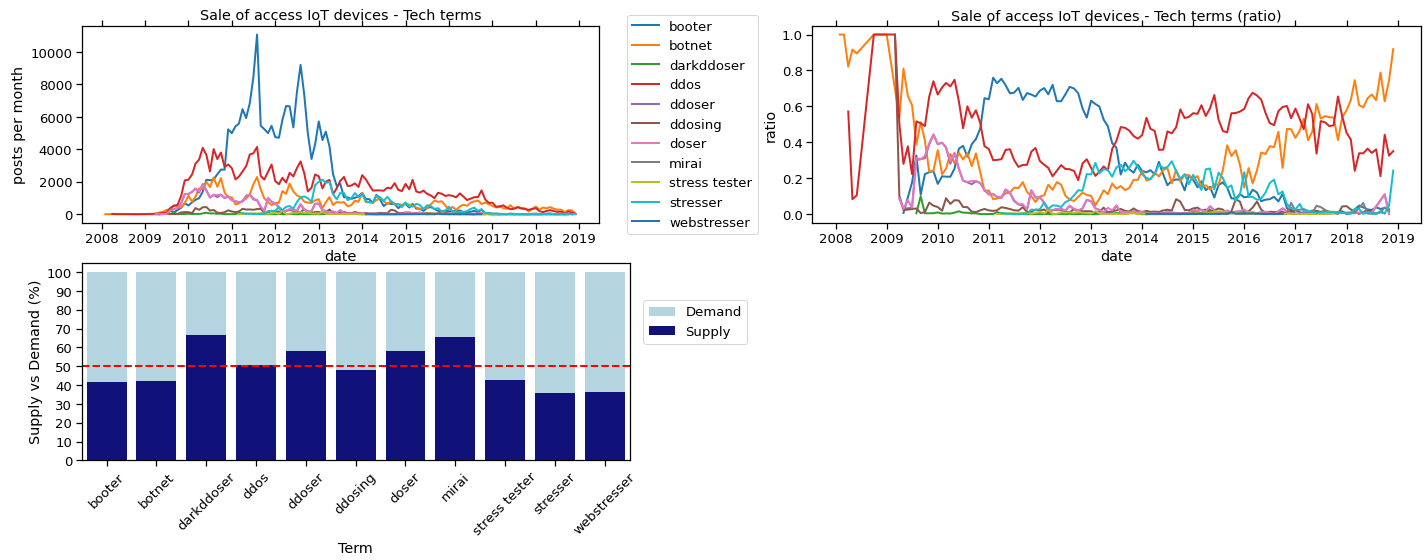
\includegraphics[width=1.0\textwidth]{figs/terms.png}
	\caption{Sale of access IoT devices - DDoS Tech terms}
	\label{fig:terms}
\end{figure}

\subsection{Preferred payment methods}

Fig. \ref{fig:payment_methods} shows how preferred payment methods, used for the Sale of access IoT devices, have evolved in last years. It is a key point in order to understand economics behind that type of criminal services.

\begin{figure}[H]
	\centering
	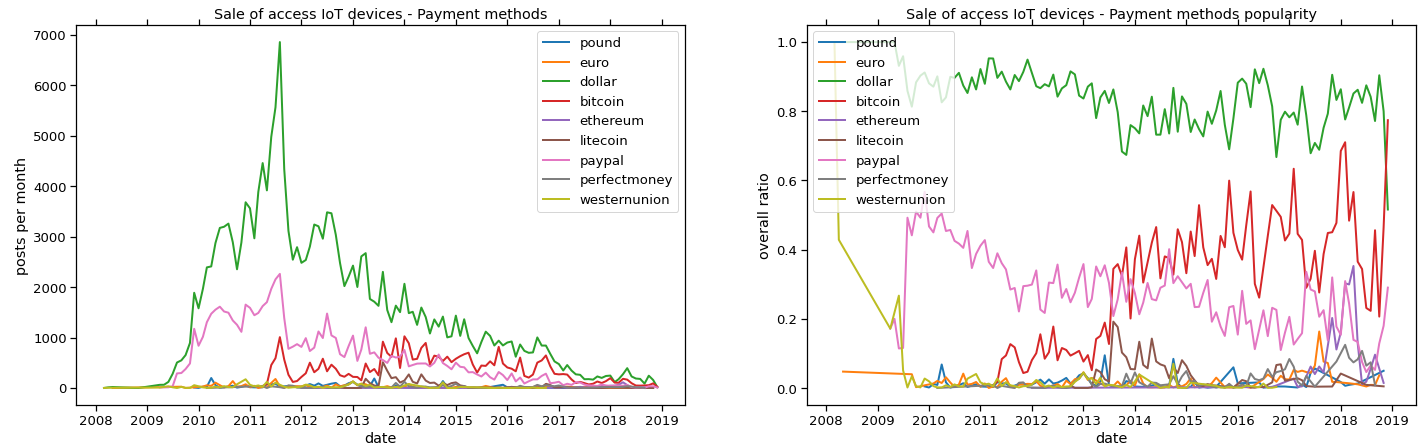
\includegraphics[width=1.0\textwidth]{figs/payment_methods.png}
	\caption{Preferred payment methods}
	\label{fig:payment_methods}
\end{figure}

The use of bitcoin as a preferred payment method has grown strongly in recent years. 